% defer/rcuintro.tex

\subsection{Introduction to RCU}
\label{sec:defer:Introduction to RCU}

앞의 섹션들에서 이야기된 방법들은 어느정도 확장성 있긴 했지만 모두 Pre-BSD
라우팅 테이블을 위한 성능에 있어서 이상적이지 못했습니다.
따라서, ``너무 멀리 가 본 자들만이 당신이 얼마나 멀리 갈 지 알 수
있다''\footnote{T.~S.~Eliot 에게의 사죄와 함께.} 정신에 의거해서, 우린 모든
방법을 알아보고, 동시의 읽기 쓰레드들이 동시의 업데이트가 존재함에도 불구하고
싱글쓰레드 탐색에서와 동일한 어셈블리어 인스트럭션들만을 수행하는 알고리즘을
들여다 볼 겁니다.
물론, 이 칭찬받아 마땅한 목표는 심각한 구현상의 의문을 일으킬 겁니다만, 시도도
해보지 않고는 성공할 수 없습니다!
\iffalse

The approaches discussed in the preceding sections have provided
some scalability but decidedly non-ideal performance for the
Pre-BSD routing table.
Therefore, in the spirit of ``only those who have gone too far
know how far you can go'',\footnote{
	With apologies to T.~S.~Eliot.}
we will go all the way, looking into algorithms in which concurrent
readers execute the same sequence of assembly language instructions as
would a single-threaded lookup, despite the presence of concurrent
updates.
Of course, this laudable goal might raise serious implementability
questions, but we cannot possibly succeed if we don't even try!
\fi

\subsubsection{Minimal Insertion and Deletion}
\label{sec:defer:Minimal Insertion and Deletion}

\begin{figure}[tb]
\begin{center}
\resizebox{3in}{!}{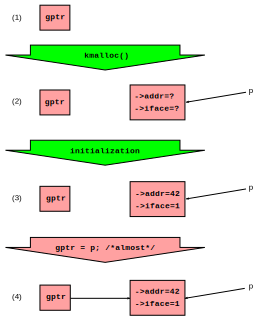
\includegraphics{defer/RCUListInsertClassic}}
\end{center}
\caption{Insertion With Concurrent Readers}
\label{fig:defer:Insertion With Concurrent Readers}
\end{figure}

구현에 있어 고려해야 할 점들을 최소화 하기 위해, 우리는 그 값이 \co{NULL}
이거나 하나의 구조체로의 레퍼런스를 갖게 되는 하나의 전역 포인터로 구성되는
최소한의 데이터 구조를 생각해 봅니다.
흥미롭게도, 이 간단한 데이터 구조는 상품에서도
사용되었습니다~\cite{GeoffRomer2018C++DeferredReclamationP0561R4}.
\iffalse

To minimize implementability concerns, we focus on a minimal
data structure, which consists of a single global pointer that is either
\co{NULL} or references a single structure.
Interestingly enough, this simple data structure is used in
production~\cite{GeoffRomer2018C++DeferredReclamationP0561R4}.
\fi

아이템 추가를 위한 고전적인 방법이
Figure~\ref{fig:defer:Insertion With Concurrent Readers} 에 표현되어 있습니다.
첫번째 열은 기본 상태를 보이는데, \co{gptr} 은 \co{NULL} 값을 갖습니다.
두번째 열에서는 하나의 구조체를 메모리 할당하는데, 초기화 되지 않은 부분들은
물음표로 표시되어 있습니다.
세번째 열에서는 이 구조체를 초기화 시킵니다.
우린 간단한 C-언어 값 할당문을 사용해서 \co{gptr} 이 이 새 원소를 가리키도록
해서, 네번째와 다섯번째 열에 보인 상태를 만들 수도 있습니다.
불행히도, Section~\ref{sec:toolsoftrade:Shared-Variable Shenanigans} 은 이
희망을 꺾습니다.
따라서, 업데이트 쓰레드는 간단한 C-언어 할당문을 사용할 수 없고, 대신
\co{smp_store_release()} 또는 나중에 설명되겠지만 \co{rcu_assign_pointer()} 를
사용해야만 합니다.
\iffalse

A classic approach for insertion is shown in
Figure~\ref{fig:defer:Insertion With Concurrent Readers}.
The first row shows the initial state, with \co{gptr} equal to \co{NULL}.
In the second row, we have allocated a structure which is uninitialized,
as indicated by the question marks.
In the third row, we have initialized the structure.
We might hope to assign \co{gptr} to reference this new element
using a simple C-language assignment statement, resulting in the
state shown in the fourth and final row.
Unfortunately, a quick review of
Section~\ref{sec:toolsoftrade:Shared-Variable Shenanigans}
dashes these hopes.
Therefore, the updater cannot use a simple C-language assignment, but
must instead use something like \co{smp_store_release()}, or, as will be seen,
\co{rcu_assign_pointer()}.
\fi

비슷하게, 어떤 사람은 읽기 쓰레드가 \co{gptr} 의 값을 읽어오는데 간단한 C-언어
값 할당문을 사용할 수도 있고, 그럼으로써 예전 값인 \co{NULL} 또는 새로 설치된
포인터를 가져오는 모두 합법적인 결과를 보장할 수도 있다고 희망할 수 있을
겁니다.
불행히도, Section~\ref{sec:toolsoftrade:Shared-Variable Shenanigans} 역시 이
희망을 꺾습니다.
이 보장을 갖기 위해선, 읽기 쓰레드들이 \co{READ_ONCE()} 또는, 뒤에서
설명하겠지만 \co{rcu_dereference()} 를 사용해야만 합니다.
하지만, 대부분의 최신 컴퓨터 시스템에서, 이 두 기능은 하나의 로드
인스트럭션으로 구현될 수 있는데, 이는 싱글쓰레드 코드에서 사용될 인스트럭션과
정확히 동일합니다.
\iffalse

Similarly, one might hope that readers could use a single C-language
assignment statement to fetch the value of \co{gptr}, and be guaranteed
to either get the old value of \co{NULL} or to get the newly installed
pointer, but either way see a valid result.
Unfortunately, Section~\ref{sec:toolsoftrade:Shared-Variable Shenanigans}
also dashes these hopes.
To obtain this guarantee, readers must instead use \co{READ_ONCE()},
or, as will be seen, \co{rcu_dereference()}.
However, on most modern computer systems, each of these two primitives
can be implemented with a single load instruction, exactly the instruction
that would be used in single-threaded code.
\fi

따라서, 이 심각한 구현상의 질문에도 불구하고, 동시의 읽기 쓰레드가 싱글쓰레드
코드에 필요시 되는 것과 동일한 기계 명령만을 수행하면서 연결된 데이터 구조에
새로운 데이터를 추가하는게 정말 가능합니다.
동시의 읽기에 추가 비용이 들지 않는 이 방법은 훌륭한 성능과 확장성을 제공하고,
real-time 사용 예에 무척 잘 맞습니다.
\iffalse

Therefore, despite the serious implementability questions, it really
is possible to add new data to linked data structures while allowing
concurrent readers to execute the same sequence of machine instructions
that is required in single-threaded code.
This no-cost approach to concurrent reading provides excellent performance
and scalability, and also is eminently suitable for real-time use.
\fi

\begin{figure}[tb]
\centering
\resizebox{3in}{!}{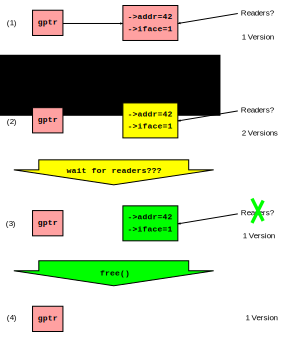
\includegraphics{defer/RCUListDeleteClassic}}
\caption{Deletion With Concurrent Readers}
\label{fig:defer:Deletion With Concurrent Readers}
\end{figure}

하지만 동시에 읽기 쓰레드에 의해 레퍼런스 되고 있는 데이터는 언젠가는 없어져야
할 겁니다.
Figure~\ref{fig:defer:Deletion With Concurrent Readers} 에 보인 것처럼, 첫번째
단계는 쉽습니다.
Section~\ref{sec:toolsoftrade:Shared-Variable Shenanigans} 에서의 교훈을 가슴에
담아서, 그 포인터를 \co{NULL} 로 만드는 데 \co{WRITE_ONCE()} 를 사용해서, 이
그림의 첫번째 줄에서 두번째 줄로 넘어갑니다.
이 시점에서, 이전부터 존재한 읽기 쓰레드들은 \co{->addr} 값은 42 이고
\co{->iface} 는 1인 이전 구조체를 보게 되지만, 새로운 읽기 쓰레드들은 \co{NULL}
포인터를 보게 되는데, 즉, 동시의 읽기 쓰레드들이 상태에 동의하지 않을 수
있으며, 이게 그림 상의 ``2 Versions'' 라고 표시되어 있습니다.
\iffalse

But sooner or later, it will be necessary to remove data that is
being referenced by concurrent readers.
As can be seen in
Figure~\ref{fig:defer:Deletion With Concurrent Readers},
the first step is easy.
Taking the lessons from
Section~\ref{sec:toolsoftrade:Shared-Variable Shenanigans}
to heart, use \co{WRITE_ONCE()} to \co{NULL} the pointer,
thus moving from the first row to the second in the figure.
At this point, pre-existing readers will see the old structure with
\co{->addr} of 42 and \co{->iface} of 1, but new readers will see
a \co{NULL} pointer, that is, concurrent readers can disagree on
the state, as indicated by the ``2 Versions'' in the figure.
\fi

\QuickQuiz{}
	Figure~\ref{fig:defer:Deletion With Concurrent Readers}
	의 \co{WRITE_ONCE()} 는 \co{smp_store_release()} 가 되어야 하지
	않을까요?
	\iffalse

	Shouldn't
	Figure~\ref{fig:defer:Deletion With Concurrent Readers}'s
	\co{WRITE_ONCE()} instead be \co{smp_store_release()}?
	\fi
\QuickQuizAnswer{
	아뇨, 그렇지 않습니다.
	\iffalse

	No, it need not be.
	\fi

	\co{NULL} 포인터가 할당되었으므로, 순서를 엇갈리게 할 것이 존재치
	않으니 \co{smp_store_release()} 는 필요가 없습니다.
	반대로, \co{NULL} 이 아닌 포인터를 할당할 때에는
	\co{smp_store_release()} 가 사용되어야 하는데 가리켜지는 구조체의
	초기화가 이 포인터 할당 전에 완료되었을 것을 보장하기 위함입니다.
	하지만 이 경우에, \co{NULL} 포인터는 가리켜지는 구조체가 없음을
	의미하므로, 순서가 필요없습니다.

	요약해서, \co{smp_store_release()} 로도 동작할 겁니다만, 불필요한
	오버헤드를 일으킬 수 있습니다.
	\iffalse

	Because a \co{NULL} pointer is being assigned, there is nothing
	to order against, so no need for \co{smp_store_release()}.
	In contrast, when assigning a non-\co{NULL} pointer, it is
	necessary to use \co{smp_store_release()} in order to ensure
	that initialization of the pointed-to structure is carried
	out before assignment of the pointer.
	But in this case, the \co{NULL} pointer means that there is
	no pointed-to structure, and thus no need for ordering.

	In short, \co{smp_store_release()} would work, but could
	incur unnecessary overhead.
	\fi
} \QuickQuizEnd

\QuickQuiz{}
	Figure~\ref{fig:defer:Deletion With Concurrent Readers}
	에 표시된 진행과 서로 동시 수행되는 읽기 쓰레드들은 \co{gptr} 의 값에
	대해 동의하지 않을 수 있습니다.
	이건 문제가 되지 않나요???
	\iffalse

	Readers running concurrently each other and with the procedure
	outlined in
	Figure~\ref{fig:defer:Deletion With Concurrent Readers}
	can disagree on the value of \co{gptr}.
	Isn't that just a wee bit problematic???
	\fi
\QuickQuizAnswer{
	꼭 그렇지는 않습니다.

	Sections~\ref{sec:cpu:Hardware Optimizations}
	와~\ref{sec:cpu:Hardware Free Lunch?} 에서 힌트가 주어졌듯이, 빛의
	속도의 지연은 컴퓨터의 데이터는 항상 그 데이터가 실제로 모델링하고자
	했던 외부의 실제에 비해 낡았음을 의미합니다.
	\iffalse

	Not necessarily.

	As hinted at in Sections~\ref{sec:cpu:Hardware Optimizations}
	and~\ref{sec:cpu:Hardware Free Lunch?},
	speed-of-light delays mean that a computer's data is always
	stale compared to whatever external reality that data is intended
	to model.
	\fi

	따라서 실제 세계의 알고리즘은 외부의 실제와 그 실제를 반영하는 컴퓨터
	내의 데이터 사이의 비일관성을 받아들일 수 있어야만 합니다.
	그런 알고리즘의 많은 부분은 컴퓨터 내부의 데이터 사이의 비일관성도
	어느정도 받아들일 수 있습니다.
	Section~\ref{sec:datastruct:RCU-Protected Hash Table Discussion}
	에서 이를 좀 더 자세히 이야기 합니다.
	\iffalse

	Real-world algorithms therefore absolutely must tolerate
	inconsistancies between external reality and the in-computer
	data reflecting that reality.
	A significant fraction of those algorithms are also able to
	tolerate some degree of inconsistency within the in-computer
	data.
	Section~\ref{sec:datastruct:RCU-Protected Hash Table Discussion}
	discusses this point in more detail.
	\fi

	이러한, 비일관성과 낡은 데이터에 대한 내성의 필요는 RCU 에만 국한되지
	않음을 알아 두시기 바랍니다.
	이는 레퍼런스 카운트, 해저드 포인터, 시퀀스 락, 심지어 일부 락킹
	사용예에도 적용됩니다.
	예를 들어, 여러분이 락을 잡은 상태에서 뭔가를 계산하고자 하지만 이
	계산된 것을 그 락을 놓은 후에 사용하고자 한다면, 여러분은 낡은 데이터를
	사용하고 있을 수 있습니다.
	무엇보다, 그 뭔가가 계산될 때의 데이터는 그 락을 놓음과 동시에 어떻게든
	바뀔 수 있습니다.

	따라서, 그래요, RCU 읽기 쓰레드는 낡고 비일관적인 데이터를 볼 수
	있습니다만, 아니요, 이건 꼭 문제라 할수는 없습니다.
	\iffalse

	Please note that this need to tolerate inconsistent and stale
	data is not limited to RCU.
	It also applies to reference counting, hazard pointers, sequence
	locks, and even to some locking use cases.
	For example, if you compute some quantity while holding a lock,
	but use that computed quantity after releasing that lock,
	you might well be using stale data.
	After all, the data from which that quantity was computed could
	change arbitrarily as soon as the lock was released.

	So yes, RCU readers can see stale and inconsistent data, but no,
	this is not necessarily problematic.
	\fi
} \QuickQuizEnd

단순히 모든 이전부터 존재한 읽기 쓰레드가 종료되기를 기다림으로써 세번째 줄에
보인 것과 같이 하나의 버전만이 존재하는 상태로 되돌아갈 수 있습니다.
이 시점에서, 모든 미리 존재한 읽기 쓰레드는 종료되었고, 어떤 뒤의 읽기 쓰레드도
과거의 데이터 항목으로 가는 경로를 갖지 못하므로, 이를 레퍼런스 하는 읽기
쓰레드는 더이상 존재할 수 없습니다.
따라서 네번째 줄에 보여진 것처럼, 이 과거의 데이터는 해제되기에 안전합니다.
\iffalse

We get back to a single version simply by waiting for all the
pre-existing readers to complete, as shown in row~3.
At that point, all the pre-existing readers are done, and no later
reader has a path to the old data item, so there can no longer be
any readers referencing it.
It may therefore be safely freed, as shown on row~4.
\fi

따라서, 이전부터 존재한 읽기 쓰레드들이 완료되기를 기다리는 방법을 제공하면,
연결된 데이터 구조에 데이터를 추가하고 제거하는게 가능합니다, 읽기 쓰레드들이
싱글쓰레드 버전에서와 동일한 기계 명령만을 수행함에도 불구하고요!
따라서 너무 멀리 갔던게 너무 멀리 간 건 전혀 아니었던 걸수도 있습니다.

하지만 이전부터 존재한 읽기 쓰레드들이 언제 정말로 완료되었다고 말할 수
있을까요?
이 질문이 다음 섹션의 주제입니다.
\iffalse

Thus, given a way to wait for pre-existing readers to complete,
it is possible to both add data to and remove data from a linked
data structure, despite the readers executing the same sequence
of machine instructions that would be appropriate for single-threaded
execution!
So perhaps going too far was not too far after all.

But how can we tell when all of the pre-existing readers have in
fact completed?
This question is the topic of the next section.
\fi

\subsubsection{Waiting for Readers}
\label{sec:defer:Waiting for Readers}

읽기 쓰레드 대기를 레퍼런스 카운팅에 기초해서 하고 싶을 수 있지만,
Chapter~\ref{chp:Counting} 의
Figure~\ref{fig:count:Atomic Increment Scalability on Nehalem}
는 동시의 레퍼런스 카운팅은 우리가
Section~\ref{sec:defer:Reference Counting} 에서 본 것처럼 상당한 오버헤드를
초래함을 보입니다.
해저드 포인터가 이 오버헤드를 상당히 줄여주지만,
Section~\ref{sec:defer:Hazard Pointers} 에서 보여주듯, 완전 없애는 건 아닙니다.
\iffalse

It is tempting to base reader waiting on reference counting, but
Figure~\ref{fig:count:Atomic Increment Scalability on Nehalem}
in
Chapter~\ref{chp:Counting}
shows that concurrent reference counting results in extreme overhead,
as we already saw in
Section~\ref{sec:defer:Reference Counting}.
Hazard pointers profoundly reduces this overhead, but, as we saw in
Section~\ref{sec:defer:Hazard Pointers}, not to zero.
\fi

두번째 방법은 메모리 동기화는 비용이 높다는 점을 파악하고, 따라서 레지스터를
대신 사용하는 것으로, 구체적으로는 각 CPU 또는 각 쓰레드의 프로그램 카운터 (PC)
에 대한 것으로, 이로써 읽기 쓰레드에게 어떤 오버헤드도 일으키지 않을 수 있는데,
최소한 동시의 업데이트가 없다면 그렇습니다.
이 업데이트 쓰레드는 각각의 연관된 PC 를 훑어보고, 만약 그 PC 가 읽기쪽 코드에
들어있지 않다면, 그 연관된 CPU 나 쓰레드는 quiescent state 에 있음을 의미하여,
결국 새로 삭제된 데이터 원소로의 접근을 할수도 있는 모든 읽기 쓰레드가
완료되었음을 알릴 수 있습니다.
모든 CPU 또는 쓰레드의 PC 가 모든 읽기 코드의 바깥에 있음이 확인되면, 이 grace
period 가 완료된 겁니다.
이 방법은 메모리 순서 잡기, \emph{가끔은} 읽기 쓰레드로부터 수행되는 함수들,
그리고 code-motion 최적화 등의 심각한 도전 과제를 가짐을 알아 두시기 바랍니다.
그러나, 이 방법은 제품 레벨에서도 사용된다고 합니다~\cite{MikeAsh2015Apple}.
\iffalse

A second approach observes that memory synchronization is expensive,
and therefore uses registers instead, namely each CPU's or thread's
program counter (PC), thus imposing no overhead on readers, at least
in the absence of concurrent updates.
The updater polls each relevant PC, and if that PC is not within read-side
code, then the corresponding CPU or thread is within a quiescent state,
in turn signalling the completion of any reader that might have access
to the newly removed data element.
Once all CPU's or thread's PCs have been observed to be outside of any
reader, the grace period has completed.
Please note that this approach poses some serious challenges, including
memory ordering, functions that are \emph{sometimes} invoked from readers,
and ever-exciting code-motion optimizations.
Nevertheless, this approach is said to be used in
production~\cite{MikeAsh2015Apple}.
\fi

세번째 방법은 어떤 합리적 읽기 쓰레드의 수명도 넘어갈 만큼 충분히 긴 고정된
시간을 그냥 기다리는 겁니다~\cite{Jacobson93,AjuJohn95}.
이는 hard real-time 시스템에서는 매우 잘 동작할 수 있습니다만, 그보다 덜
매력적인 환경에서라면, Murphy 는 비합리적으로 긴 수명의 읽기 쓰레드에도 준비해
두는게 매우 중요하다고 말할 겁니다.
이걸 이해하기 위해, 충분히 길게 기다리는데 실패하는 경우의 결과를 생각해
보세요: 어떤 데이터 아이템은 비합리적인 읽기 쓰레드가 여전히 그걸 레퍼런스하고
있는 중에 해제되고, 그 아이템은 곧바로 재할당 되어서, 다른 타입의 데이터
아이템이 되어 있을 수도 있습니다.
이 비합리적인 읽기 쓰레드와 부주의한 재할당자는 이제 같은 메모리를 두개의 매우
다른 목적으로 사용하려 할 겁니다.
이 문제는 최선의 경우에도 무척 디버깅하기 어려울 겁니다.
\iffalse

A third approach is to simply wait for a fixed period of time that is
long enough to comfortably exceed the lifetime of any reasonable
reader~\cite{Jacobson93,AjuJohn95}.
This can work quite well in hard real-time systems, but in less exotic
settings, Murphy says that it is critically important to be prepared
even for unreasonably long-lived readers.
To see this, consider the consequences of failing to wait long enough:
A data item will be freed while the unreasonable reader is still
referencing it, and that item might well be immediately reallocated,
possibly even as a data item of some other type.
The unreasonable reader and the unwitting reallocator would then
be attempting to use the same memory for two very different purposes.
The ensuing mess will at best be exceedingly difficult to debug.
\fi

네번째 방법은 가장 비합리적인 읽기 쓰레드도 기다릴 수 있도록 영원히 기다리는
겁니다.
이 방법은 ``메모리 누출'' 이라고도 불리며, 메모리 누출은 종종 때이른 리부팅을
필요로 한다는 사실 때문에 나쁜 평판을 가지고 있습니다.
하지만, 평판에도 불구하고, 업데이트 비율과 시스템 운용 시간의 최대값이 확실히
제한되어 있는 경우에는 실행 가능한 전략입니다.
예를 들어, 클러스터가 정말로 높은 availability 를 보장함을 증명하기 위해
주기적으로 크래시 되는 높은 availability 의 클러스터에서는 잘 사용될 수도 있을
겁니다.\footnote{
	주기적인 크래시를 강제하는 이 프로그램은 가끔 ``chaos monkey'' 라고도
	알려져 있습니다:
	\url{https://netflix.github.io/chaosmonkey/}.}
메모리를 누출하는 건 또한 가비지 콜렉터가 있는 환경에서라면 실행 가능한
전략인데, 이 경우 가비지 콜렉터는 이 누출에 대한 마개가 될
겁니다~\cite{Kung80}.
하지만, 여러분의 환경이 가비지 콜렉터를 갖지 못했다면, 계속 읽으세요!
\iffalse

A fourth approach is to wait forever, secure in the knowledge that
doing so will outwait even the most unreasonable reader.
This approach is also called ``leaking memory'', and has a bad reputation
due to the fact that memory leaks often require untimely and
highly inconvenient reboots.
However, reputation notwithstanding, this is a viable strategy when
the update rate and the uptime are both sharply bounded.
For example, this approach could work well in a high-availability
cluster where systems were periodically crashed in order to ensure
that cluster really remained highly available.\footnote{
	The program that forces the periodic crashing is sometimes
	known as a ``chaos monkey'':
	\url{https://netflix.github.io/chaosmonkey/}.}
Leaking the memory is also a viable strategy in environments having
garbage collectors, in which case the garbage collector can be thought
of as plugging the leak~\cite{Kung80}.
However, if your environment lacks a garbage collector, read on!
\fi

다섯번째 방법은 주기적으로 ``모든 걸 멈추기'' 를 보다 선호함으로써 주기적
크래시를 막는데, 전통적인 stop-the-world 가비지 콜렉터로 보여지듯이 이를 잘
보입니다.
하지만, 오늘날의 모든게 연결되고 모든게 켜져있는 세계에서, 모든 걸 멈추기는
응답 시간을 상당히 악화시킬 수 있는데, 이는 동시적 가비지
콜렉터~\cite{DavidFBacon2003RTGC}의 개발에 대한 모티베이션이 되었습니다.
더 나아가서, 우린 모든 이전부터 존재한 읽기 쓰레드들이 완료되길 원하지, 모든게
한번에 완료되길 바라는 건 아닙니다.
\iffalse

A fifth approach avoids the period crashes in favor of periodically
``stopping the world'', as exemplified by the traditional stop-the-world
garbage collector.
This approach was also heavily used during the decades before
ubiquitous connectivity, when it was common practice to power systems
off at the end of each working day.
However, in today's always-connected always-on world, stopping the world
can gravely degrade response times, which has been one motivation for the
development of concurrent garbage collectors~\cite{DavidFBacon2003RTGC}.
Furthermore, we only need all pre-existing readers to complete, not to
complete all at the same time.
\fi

이 관찰은 여섯번째 방법을 이끄는데, 하나의 CPU 또는 쓰레드를 충분한 시간동안
멈추는 것입니다.
이 방법은 읽기 쓰레드의 응답 시간을 전혀 악화시키지 않고, 멈춰진 하나의 것의
응답시간만 악화시킵니다.
더 나아가서, 다양한 어플리케이션이 이미 모든 이전부터 존재한 읽기 쓰레드들이
완료된 후에야 도달 가능한 상태 (\emph{quiescent state}) 를 가지고 있습니다.
트랜잭션 처리 시스템에서, 한쌍의 성공적인 트랜잭션 사이의 시간이 하나의
quiescent state 가 될 수 있습니다.
Preemption 을 제공하지 않는 운영체제 커널에서, 컨텍스트 스위치는 하나의
quiescent state 가 될 수 있습니다~\cite{McKenney98}.
어느 쪽이던, 모든 CPU 그리고/또는 쓰레드들이 하나의 quiescent state 를
지났다면, 이 시스템은 하나의 \emph{grace period} 를 완료했다고, 모든 이전부터
존재한 읽기 쓰레드들이 완료되었다고 말해지며, 모든 이전에 제거된 데이터
아이템이 해제되기에 안전하다고 말해집니다.\footnote{
	단순히 메모리 회수를 지연시키는 것보다 RCU 는 더 많은 걸 할 수
	있습니다만, 메모리 회수 지연은 시작하기에 좋은 내용입니다.}
\iffalse

This observation leads to the sixth approach, which is stopping
one CPU or thread at a time.
This approach has the advantage of not degrading reader response times
at all, let alone gravely.
Furthermore, numerous applications already have states (termed
\emph{quiescent states}) that can be
reached only after all pre-existing readers are done.
In transaction-processing systems, the time between a pair of
successive transactions might be a quiescent state.
In reactive systems, the state between a pair of successive events
might be a quiescent state.
Within non-preemptive operating-systems kernels, a context switch can be
a quiescent state~\cite{McKenney98}.
Either way, one all CPUs and/or threads have passed through a quiescent
state, the system is said to have completed a \emph{grace period},
such that all pre-existing readers have completed, and it is now
safe to free any previously-removed data items.\footnote{
	It is possible to do much more with RCU than simply defer
	reclamation of memory, but deferred reclamation is an
	excellent place to start.}
\fi

Preemption 을 하지 않는 운영체제 커널에서, 컨텍스트 스위치가 합법적 quiescent
state 가 되기 위해선, 읽기 쓰레드들이
Figure~\ref{fig:defer:Insertion With Concurrent Readers}
와~\ref{fig:defer:Deletion With Concurrent Readers} 에 보여진 \co{gptr} 를 통해
얻어온 특정 데이터 자료의 인스턴스를 레퍼런스 하는 동안 블록되는걸 금지해야만
합니다.
이 블록킹 금지 규칙은 스핀락을 잡고 있는 동안은 CPU 가 블록되는게 금지되는 순수
스핀락과 같은 비슷한 규칙입니다.
이 금지 규칙이 없으면, 모든 CPU 가 블락된 쓰레드가 잡고있는 스핀락을 잡고자
스피닝 하는 쓰레드들에 의해 소모될 수 있습니다.
이 스피닝 하는 쓰레드들은 각자가 이 락을 획득하기 전까지는 CPU 를 놓지 않을
것인데, 이 락을 잡고 있는 쓰레드는 이 스피닝 하는 쓰레드들 중 하나가 CPU 를
놓기 전까지는 락을 놓을 수가 없습니다.
이는 고전적인 데드락 상황이며, 이 데드락은 스핀락을 잡고 있는 동안은 블록되는
것을 금지하는 것으로 막아집니다.
\iffalse

Within a non-preemptive operating-system kernel, for context switch to be
a valid quiescent state, readers must be prohibited from blocking while
referencing a given instance data structure obtained via the \co{gptr}
pointer shown in
Figures~\ref{fig:defer:Insertion With Concurrent Readers}
and~\ref{fig:defer:Deletion With Concurrent Readers}.
This no-blocking constraint is consistent with similar constraints
on pure spinlocks, where a CPU is forbidden from blocking while
holding a spinlock.
Without this prohibition, all CPUs might be consumed by threads
spinning attempting to acquire a spinlock held by a blocked thread.
The spinning threads will not relinquish their CPUs until they acquire
the lock, but the thread holding the lock cannot possibly release it
until one of the spinning threads relinquishes a CPU.
This is a classic deadlock situation, and this deadlock is avoided
by prohibiting blocking while holding a spinlock.
\fi

다시 말하지만, 이 동일한 금지 규칙은 \co{gptr} 을 디레퍼런싱하는 읽기
쓰레드들에 부과됩니다: 그런 쓰레드들은 그 포인터로 가리켜진 데이터 아이템을
사용하는 걸 마무리 하기 전까지는 블록될 수 없습니다.
업데이트 쓰레드가 \co{WRITE_ONCE()} 를 수행하는 걸 마무리 한
Figure~\ref{fig:defer:Deletion With Concurrent Readers} 의 두번째 줄로
돌아와서, CPU~0 이 컨텍스트 스위치를 한다고 생각해 봅시다.
읽기 쓰레드들은 이 링크드 리스트를 횡단하는 동안 블록되는게 허용되어 있지
않으므로, CPU~0 에서 수행된 모든 이전의 읽기 쓰레드는 완료되었다고 보장됩니다.
이 논리를 다른 CPU 들에도 적용해 보면, 일단 모든 CPU 들이 컨텍스트 스위치를
수행했음이 관측되었다면, 모든 이전의 읽기 스레드들이 완료되었으며, 따라서 새로
제거된 데이터 원소를 레퍼런스하는 읽기 쓰레드는 더이상 존재하지 않는다는게
보장됩니다.
이 업데이트 쓰레드는 이제 안전하게 이 데이터 원소를 해제할 수 있어서,
Figure~\ref{fig:defer:Deletion With Concurrent Readers} 의 바닥에 보여진 상태를
이룰 수 있습니다.
\iffalse

Again, this same constraint is imposed on reader threads dereferencing
\co{gptr}: such threads are not allowed to block until after
they are done using the pointed-to data item.
Returning to the second row of
Figure~\ref{fig:defer:Deletion With Concurrent Readers},
where the updater has just completed executing the \co{WRITE_ONCE()},
imagine that CPU~0 executes a context switch.
Because readers are not permitted to block while traversing the linked
list, we are guaranteed that all prior readers that might have been running on
CPU~0 will have completed.
Extending this line of reasoning to the other CPUs, once each CPU has
been observed executing a context switch, we are guaranteed that all
prior readers have completed, and that there are no longer any reader
threads referencing the newly removed data element.
The updater can then safely free that data element, resulting in the
state shown at the bottom of
Figure~\ref{fig:defer:Deletion With Concurrent Readers}.
\fi

\begin{figure}[tb]
\centering
\resizebox{3in}{!}{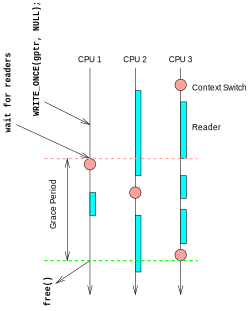
\includegraphics{defer/QSBRGracePeriod}}
\caption{QSBR: Waiting for Pre-Existing Readers}
\label{fig:defer:QSBR: Waiting for Pre-Existing Readers}
\end{figure}

이런 방법은 \emph{quiescent state based
reclamation}(QSBR)~\cite{ThomasEHart2006a} 이라 명명되어 있습니다.
QSBR 방법이
Figure~\ref{fig:defer:QSBR: Waiting for Pre-Existing Readers},
에 그림의 꼭대기부터
바닥까지로 시간의 흐름에 따라 그려져 있습니다.
CPU~1 은 현재 데이터 아이템을 제거하는 \co{WRITE_ONCE()} 를 행하고 (아마 앞서서
이 포인터 값을 읽었고 적절한 동기화를 했을 겁니다), 이어서 읽기 쓰레드들을
기다립니다.
이 기다리기 동작은 즉각적인 컨텍스트 스위치로 귀결되는데, 이는 quiescent state
로, CPU~1 위의 모든 앞의 읽기들이 완료되었음을 의미합니다.
다음으로, CPU~2 가 컨텍스트 스위치를 해서, CPU~1 과~2 의 모든 읽기 쓰레드가
완료되었음이 알려집니다.
마지막으로, CPU~3 가 컨텍스트 스위치를 합니다.
이 시점에서, 전체 시스템의 모든 읽기 쓰레드는 완료되었음이 알려진 것이고,
따라서 grace period 가 종료되어서, CPU~1 이 기존 데이터 아이템을 해제할 수 있게
됩니다.

\iffalse
This approach is termed \emph{quiescent state based reclamation}
(QSBR)~\cite{ThomasEHart2006a}.
A QSBR schematic is shown in
Figure~\ref{fig:defer:QSBR: Waiting for Pre-Existing Readers},
with time advancing from the top of the figure to the bottom.
CPU~1 does the \co{WRITE_ONCE()} that removes the current data
item (presumably having previously read the pointer value and
availed itself of appropriate synchronization), then waits
for readers.
This wait operation results in an immediate context switch, which is
a quiescent state, which in turn means that all prior reads on CPU~1
have completed.
Next, CPU~2 does a context switch, so that all readers on CPUs~1 and~2
are now known to have completed.
Finally, CPU~3 does a context switch.
At this point, all readers throughout the entire system are known to
have completed, so the grace period ends, permitting CPU~1 to free
the old data item.
\fi

\QuickQuiz{}
	Figure~\ref{fig:defer:QSBR: Waiting for Pre-Existing Readers} 에서,
	과거의 데이터 아이템에 접근했을 수도 있는 CPU~3 의 마지막 읽기 쓰레드는
	grace period 가 시작하기 전에 이미 종료되었습니다!
	그런데 왜 CPU~3 가 이후의 컨텍스트 스위치를 할 때까지 기다리는거죠???
	\iffalse

	In Figure~\ref{fig:defer:QSBR: Waiting for Pre-Existing Readers},
	the last of CPU~3's readers that could possibly have
	access to the old data item ended before the grace period
	even started!
	So why would any anyone bother waiting until CPU~3's later context
	switch???
	\fi
\QuickQuizAnswer{
	이 기다림이 바로 읽기 쓰레드가 싱글쓰레드의 경우와 동일한 인스트럭션을
	수행할 수 있도록 해주는 것이기 때문입니다.
	달리 말하자면, 기다림이 훌륭한 읽기쪽 성능, 확장성, 그리고 real-time
	응답을 가능하게 합니다.
	\iffalse

	Because that waiting is exactly what enables readers to use
	the same sequence of instructions that is appropriate for
	single-theaded situations.
	In other words, waiting enables excellent read-side performance,
	scalability, and real-time response.
	\fi
} \QuickQuizEnd

\subsubsection{Toy Implementation}
\label{sec:defer:Toy Implementation}

제품 수준 QSBR 구현은 상당히 복잡할 수 있지만, 비선점 모드 리눅스 커널에서의
장난감 수준 구현은 상당히 간단합니다:
\iffalse

Although production-quality QSBR implementations can be quite complex,
a toy non-preemptive Linux-kernel implementation is exceedingly simple:
\fi

\begin{VerbatimN}[samepage=true]
void synchronize_rcu(void)
{
	int cpu;

	for_each_online_cpu(cpu)
		run_on(cpu);
}
\end{VerbatimN}

이 \co{for_each_online_cpu()} 함수는 모든 CPU 들에 루프를 돌고, \co{run_on()}
함수는 현재 쓰레드가 특정 CPU 에서 수행되게 해서 목적지 CPU 가 컨텍스트
스위칭을 수행하게 만듭니다.
따라서, 일단 한번 \co{for_each_online_cpu()} 가 완료되면, 각 CPU 는 컨텍스트
스위치를 수행한 것이고, 따라서 모든 시간상 앞의 읽기 쓰레드들은 완료되었음이
보장됩니다.
\iffalse

The \co{for_each_online_cpu()} primitive iterates over all CPUs, and
the \co{run_on()} function causes the current thread to execute on the
specified CPU, which forces the destination CPU to execute a context
switch.
Therefore, once the \co{for_each_online_cpu()} has completed, each CPU
has executed a context switch, which in turn guarantees that
all pre-existing reader threads have completed.
\fi

이 방법은 제품 수준의 품질이 \emph{아님} 을 알아 두시기 바랍니다.
일반적이지 않은 경우에서의 정확성 처리와 강력한 최적화 여럿을 필요로 하는 제품
수준 품질의 구현의 성질은 상당한 추가적 복잡도를 의미합니다.
또한, CPU 강탈이 가능한 환경에서의 RCU 구현은 읽기 쓰레드들이 실제로 뭔가를
할것을 필요로 합니다.
하지만, 이 간단한 CPU 강탈이 불가한 상황의 접근법은 개념적으로는 완벽하고, 다음
섹션에서 다루어질 RCU 의 기본을 이해하기 위한 좋은 초기 토대가 될겁니다.

\begin{listing}[tbp]
{ \scriptsize
\begin{verbbox}[\LstLineNo]
struct route *gptr;

int access_route(int (*f)(struct route *rp))
{
  int ret = -1;
  struct route *rp;

  rcu_read_lock();
  rp = rcu_dereference(gptr);
  if (rp)
  	ret = f(rp);
  rcu_read_unlock();
  return ret;
}

struct route *ins_route(struct route *rp)
{
  struct route *old_rp;

  spin_lock(&route_lock);
  old_rp = gptr;
  rcu_assign_pointer(gptr, rp);
  spin_unlock(&route_lock);
}

int del_route(void)
{
  struct route *old_rp;

  spin_lock(&route_lock);
  old_rp = gptr;
  RCU_INIT_POINTER(gptr, NULL);
  spin_unlock(&route_lock);
  synchronize_rcu();
  free(old_rp);
  return !!old_rp;
}
\end{verbbox}
}
\centering
\theverbbox
\caption{Insertion and Deletion With Concurrent Readers}
\label{lst:defer:Insertion and Deletion With Concurrent Readers}
\end{listing}

이 방법은 제품 수준이 \emph{아님} 에 유의해 주시기 바랍니다.
여러 코너 케이스의 올바른 처리와 여러 강력한 최적화의 필요는 제품 수준 구현은
상당한 추가적 복잡성을 가짐을 의미합니다.
또한, 선점이 가능한 환경에서의 RCU 구현은 읽기 쓰레드들이 실제로 뭔가를 행할
것을 필요로 합니다.\footnote{
	선점 가능 환경을 위한 일부 장난감 수준 RCU 구현은
	Appendix~\ref{chp:app:``Toy'' RCU Implementations} 에서 볼 수
	있습니다.}
하지만, 이 간단한 선점 불가 환경 방법은 개념적으로 완벽하고, 동시의 업데이트가
있는 상황에서도 read-side 동기화를 비용 없이 가능하게 함을 보입니다.
실제로,
Listing~\ref{lst:defer:Insertion and Deletion With Concurrent Readers}
은 읽기를 하는 방법을 (\co{access_route()}),
Figure~\ref{fig:defer:Insertion With Concurrent Readers}
의 삽입 (\co{ins_route()}) 과
Figure~\ref{fig:defer:Deletion With Concurrent Readers}
의 삭제 (\co{del_route()} 가 구현될 수 있는지 보입니다.
(조금 더 쓸만한 라우팅 테이블은
Section~\ref{sec:defer:RCU for Pre-BSD Routing} 에 보여져 있습니다.)
\iffalse

Please note that this approach is \emph{not} production quality.
Correct handling of a number of corner cases and the need for a number
of powerful optimizations mean that production-quality implementations
have significant additional complexity.
In addition, RCU implementations for preemptible environments
require that readers actually do something.\footnote{
	Some toy RCU implementations that handle preemptive
	environments are shown in
	Appendix~\ref{chp:app:``Toy'' RCU Implementations}.}
However, this simple non-preemptible approach is conceptually complete,
and demonstrates that it really is possible to provide read-side
synchronization at zero cost, even in the face of concurrent updates.
In fact,
Listing~\ref{lst:defer:Insertion and Deletion With Concurrent Readers}
shows how reading (\co{access_route()}),
Figure~\ref{fig:defer:Insertion With Concurrent Readers}'s
insertion (\co{ins_route()}) and
Figure~\ref{fig:defer:Deletion With Concurrent Readers}'s
deletion (\co{del_route()}) can
be implemented.
(A slightly more capable routing table is shown in
Section~\ref{sec:defer:RCU for Pre-BSD Routing}.)
\fi

\QuickQuiz{}
	Listing~\ref{lst:defer:Insertion and Deletion With Concurrent Readers}
	의 \co{rcu_read_lock()} 과 \co{rcu_read_unlock()} 의 요점이 뭐죠?
	그냥 quiescent state 들이 그것들을 이야기 하도록 두지 않는 이유가 뭐죠?
	\iffalse

	What is the point of \co{rcu_read_lock()} and \co{rcu_read_unlock()} in
	Listing~\ref{lst:defer:Insertion and Deletion With Concurrent Readers}?
	Why not just let the quiescent states speak for themselves?
	\fi
\QuickQuizAnswer{
	읽기 쓰레드들은 quiescent state 를 넘어다니지 못하게 되어 있음을 다시
	말씀드립니다.
	예를 들어, 리눅스 커널에서, RCU 읽기 쓰레드는 컨텍스트 스위치를 수행할 수 없습니다.
	\co{rcu_read_lock()} 과 \co{rcu_read_unlock()} 의 사용은 올바르지 않게
	위치한 quiescent state 를 위한 디버깅 목적의 검사를 가능하게 해서,
	그렇지 않다면 찾기 어렵고, 간헐적으로 발생하며, 상당히 파괴적인
	버그들을 찾기 쉽게 해줍니다.
	\iffalse

	Recall that readers are not permitted to pass through a quiescent
	state.
	For example, within the Linux kernel, RCU readers are not permitted
	to execute a context switch.
	Use of \co{rcu_read_lock()} and \co{rcu_read_unlock()} enables
	debug checks for improperly placed quiescent states, making it
	easy to find bugs that would otherwise be difficult to find,
	intermittent, and quite destructive.
	\fi
} \QuickQuizEnd

\QuickQuiz{}
	Listing~\ref{lst:defer:Insertion and Deletion With Concurrent Readers}
	의 \co{rcu_dereference()}, \co{rcu_assign_pointer()}, 그리고
	\co{RCU_INIT_POINTER()} 의 의미는 뭐죠?
	왜 그냥 \co{READ_ONCE()}, \co{smp_store_release()}, 그리고
	\co{WRITE_ONCE()} 를 대신 사용하지 않는 건가요?
	\iffalse

	What is the point of \co{rcu_dereference()}, \co{rcu_assign_pointer()}
	and \co{RCU_INIT_POINTER()} in
	Listing~\ref{lst:defer:Insertion and Deletion With Concurrent Readers}?
	Why not just use \co{READ_ONCE()}, \co{smp_store_release()}, and
	\co{WRITE_ONCE()}, respectively?
	\fi
\QuickQuizAnswer{
	이 RCU 를 위한 API 들은 제안된 대안들과 비슷한 의미를 갖습니다만, RCU
	를 위한 API 들이 RCU 와 관련 없는 곳에서 사용되었거나 그 반대인 경우를
	파악해내는 정적 분석 기반 디버깅을 가능하게 합니다.
	\iffalse

	The RCU-specific APIs do have similar semantics to the suggested
	replacements, but also enable static-analysis debugging checks
	that complain if an RCU-specific API is invoked on a non-RCU
	pointer and vice versa.
	\fi
} \QuickQuizEnd

Listing~\ref{lst:defer:Insertion and Deletion With Concurrent Readers}
으로 돌아가서, \co{route_lock} 은 \co{ins_route()} 와 \co{del_route()} 를
호출하는 동시적인 업데이트 쓰레드들 사이의 동기화를 위해 사용됨을 알아두시기
바랍니다.
하지만, 이 락은 \co{access_route()} 를 호출하는 읽기 쓰레드에 의해 잡히지
않습니다:
읽기 쓰레드들은 이 섹션에서 설명한 QSBR 기법을 통해 보호됩니다.

\co{ins_route()} 는 단순히
Figure~\ref{fig:defer:Insertion With Concurrent Readers} 에서 항상 \co{NULL} 일
것이라 가정된 \co{gptr} 의 과거 값을 리턴함을 알아두시기 바랍니다.
이는 \co{NULL} 이 아닌 값을 가지고 무얼 할지는 호출자의 책임으로, 이 작업은
읽기 쓰레드들이 한동안 그 값을 계속 레퍼런스 하고 있다는 사실로 인해 복잡해
집니다.
호출자들은 아래 방법들 중 하나를 사용할 수 있을 겁니다:
\iffalse

Referring back to
Listing~\ref{lst:defer:Insertion and Deletion With Concurrent Readers},
note that \co{route_lock} is used to synchronize between concurrent updaters
invoking \co{ins_route()} and \co{del_route()}.
However, this lock is not acquired by readers invoking \co{access_route()}:
Readers are instead protected by the QSBR techniques described in this section.

Note that \co{ins_route()} simply returns the old value of \co{gptr}, which
Figure~\ref{fig:defer:Insertion With Concurrent Readers} assumed would
always be \co{NULL}.
This means that it is the caller's responsibility to figure out what to
do with a non-\co{NULL} value, a task complicated by the fact that
readers might still be referencing it for an indeterminate period of time.
Callers might use one of the following approaches:
\fi

\begin{enumerate}
\item	가리켜지는 구조체를 안전히 해제시키기 위해 \co{synchronize_rcu()} 를
	사용합니다.
	이 방법이 RCU 관점에서 올바르지만, 소프트웨어 엔지니어링 관점에서
	누출되는 API 문제를 가질 수도 있습니다.
\item	리턴된 포인터가 \co{NULL} 이 아닌 경우를 위한 단정문을 집어넣습니다.
\item	이전의 값을 복구하기 위해 리턴된 포인터를 향후의 \co{ins_route()}
	호출에 넘깁니다.
\iffalse

\item	Use \co{synchronize_rcu()} to safely free the pointed-to structure.
	Although this approach is correct from an RCU perspective, it
	arguably has software-engineering leaky-API problems.
\item	Trip an assertion if the returned pointer is non-\co{NULL}.
\item	Pass the returned pointer to a later invocation of
	\co{ins_route()} to restore the earlier value.
\fi
\end{enumerate}

대조적으로, \co{del_route()} 는 새로 삭제된 데이터 항목을 안전히 해제시키기
위해 \co{synchronize_rcu()} 와 \co{free()} 를 사용합니다.

이 예제는 RCU 로 보호되는 데이터 구조들을 읽고 업데이트하는 일반적인 한가지
방법을 보입니다만, 상당히 다양한 사용 예가 있을 수 있으며, 그 중 몇가지는
Section~\ref{sec:defer:RCU Usage} 에서 다뤄집니다.

요약하자면, 싱글쓰레드 환경에서 읽기 쓰레드들이 수행할 것과 똑같은 기계
명령어만을 수행하는 읽기 쓰레드에 의해 횡단될 수 있으며 동시의 여러 쓰레드가
접근할 수 있는 연결된 데이터 구조를 만드는게 가능합니다.
다음 섹션은 RCU 의 고수준 특성들을 요약합니다.
\iffalse

In contrast, \co{del_route()} uses \co{synchronize_rcu()} and
\co{free()} to safely free the newly deleted data item.

This example shows one general approach to reading and updating
RCU-protected data structures, however, there is quite a variety
of use cases, several of which are covered in
Section~\ref{sec:defer:RCU Usage}.

In summary, it is in fact possible to create concurrent linked data
structures that can be traversed by readers executing the same sequence
of machine instructions that would be executed by single-threaded readers.
The next section summarizes RCU's high-level properties.
\fi

\subsubsection{RCU Properties}
\label{sec:defer:RCU Properties}

RCU 는 읽기가 업데이트와 동시에 유용한 진행을 할 수 있게 함으로써 확장성을
개선하는데, 업데이트도 유용한 진행을 할 수 있게 해줍니다.
이 특성은 RCU 구현이 낮은 비용의 또는 심지어 비용이 없는 읽기 쓰레드를 가능하게
하는데, 상호 배제를 제공함으로써 유용한 동시의 진행을 불가능하게 하는 일반적인
동기화 기능들과 대비됩니다.
RCU 는 \co{rcu_read_lock()} 과 \co{rcu_read_unlock()} 을 통해 읽기 쓰레드들을
구분하며 오브젝트의 여러 버전을 관리하고 오브젝트가 모든 이전부터 존재한
read-side 크리티컬 섹션이 완료되기 전에 해제되지 않았음을 보장하기 위해
\co{synchronize_rcu()} 와 같은 update-side 기능을 사용함으로써 각 읽기 쓰레드가
일관적인 시각을 확보할 수 있게 합니다.
RCU 는 오브젝트의 새로운 버전을 내보내고 읽기 위한 효율적이고 확장성 있는
메커니즘을 제공하기 위해 \co{rcu_assign_pointer()} 와 \co{rcu_dereference()} 를
각각 정의하고 사용합니다.
이 메커니즘은 읽기와 업데이트 경로의 일을 분산시키는데 읽기 경로는 해저드
포인터와 비슷하게 복제와 최적화를 최소화 시키되 읽기 쪽의 재시도를 막음으로써
극단적으로 빠르게 합니다.
일부 경우에, \co{CONFIG_PREEMPT=n} 리눅스 커널에서 RCU 의 읽기쪽 기능들은 아예
오버헤드가 없습니다.
\iffalse

RCU achieves scalability
improvements by allowing reads to make useful forward progress
concurrently with updates, which are also allowed to make useful
forward progress.
This property enables RCU implementations to provide low-cost
or even no-cost readers,
in contrast with conventional synchronization primitives that
provide mutual exclusion, thus prohibiting useful concurrent forward
progress.
RCU delimits readers with \co{rcu_read_lock()} and \co{rcu_read_unlock()},
and ensures that each reader has a coherent view by
maintaining multiple versions of objects and using update-side primitives
such as \co{synchronize_rcu()} to ensure that objects are not
freed until all pre-existing read-side critical sections complete.
RCU defines and uses \co{rcu_assign_pointer()} and \co{rcu_dereference()}
to provide efficient and scalable mechanisms for publishing
and reading new versions of an object, respectively.
These mechanisms distribute the work among read and
update paths in such a way as to make read paths extremely fast, using
replication and weakening optimizations in a manner similar to
hazard pointers, but without the need for read-side retries.
In some cases, including \co{CONFIG_PREEMPT=n} Linux kernels,
RCU's read-side primitives have zero overhead.
\fi

\QuickQuiz{}
	하지만 Section~\ref{sec:defer:Sequence Locks} 의 seqlock 또한 읽기
	쓰레드와 업데이트 쓰레드가 동시에 일을 할 수 있게 하지 않나요?
	\iffalse

	But doesn't Section~\ref{sec:defer:Sequence Locks}'s seqlock
	also permit readers and updaters to get work done concurrently?
	\fi
\QuickQuizAnswer{
	그렇고 아닙니다.
	Seqlock 읽기 쓰레드가 seqlock 쓰기 쓰레드와 동시에 수행될 수 있긴
	하지만, 그렇게 될 때마다 \co{read_seqretry()} 기능이 이 읽기 쓰레드를
	재시도 하게 강제합니다.
	이말은 seqlock 업데이트 쓰레드와 동시에 수행되는 seqlock 읽기 쓰레드가
	폐기되고 재처리될 것을 의미합니다.
	따라서 seqlock 읽기 쓰레드는 업데이트 쓰레드와 동시에 \emph{돌아갈}
	수는 있으나 이 경우 어떤 일도 실제로 하지는 못합니다.
	\iffalse

	Yes and no.
	Although seqlock readers can run concurrently with
	seqlock writers, whenever this happens, the \co{read_seqretry()}
	primitive will force the reader to retry.
	This means that any work done by a seqlock reader running concurrently
	with a seqlock updater will be discarded and redone.
	So seqlock readers can \emph{run} concurrently with updaters,
	but they cannot actually get any work done in this case.
	\fi

	반면, RCU 읽기 쓰레드는 동시의 RCU 업데이트 쓰레드가 있는 상황에서도
	유용한 일을 해낼 수 있습니다.
	\iffalse

	In contrast, RCU readers can perform useful work even in presence
	of concurrent RCU updaters.
	\fi

	하지만, 레퍼런스 카운터
	(Section~\ref{sec:defer:Reference Counting}) 도
	해저드 포인터
	(Section~\ref{sec:defer:Hazard Pointers}) 도 업데이트 쓰레드와 읽기
	쓰레드 모두 동시의 유용한 진행을 정말로 할 수 있게 합니다만 꽤 큰
	비용을 수반합니다.
	이 deferred-reclamation 문제에 대한 다른 해결책들을 비교하려면
	Section~\ref{sec:defer:Which to Choose?} 을 보시기 바랍니다.
	\iffalse

	However, both reference counters
	(Section~\ref{sec:defer:Reference Counting})
	and hazard pointers
	(Section~\ref{sec:defer:Hazard Pointers})
	really do permit useful concurrent forward progress for both
	updaters and readers, just at somewhat greater cost.
	Please see
	Section~\ref{sec:defer:Which to Choose?}
	for a comparison of these different solutions to the
	deferred-reclamation problem.
	\fi
} \QuickQuizEnd

하지만 이 기능들이 실제로 유용할까요?
이 질문에 대해선 다음 섹션에서 다룹니다.
\iffalse

But are these properties actually useful in practice?
This question is taken up by the next section.
\fi

\subsubsection{Practical Applicability}
\label{sec:defer:Practical Applicability}

\begin{figure}[tb]
\centering
\resizebox{3in}{!}{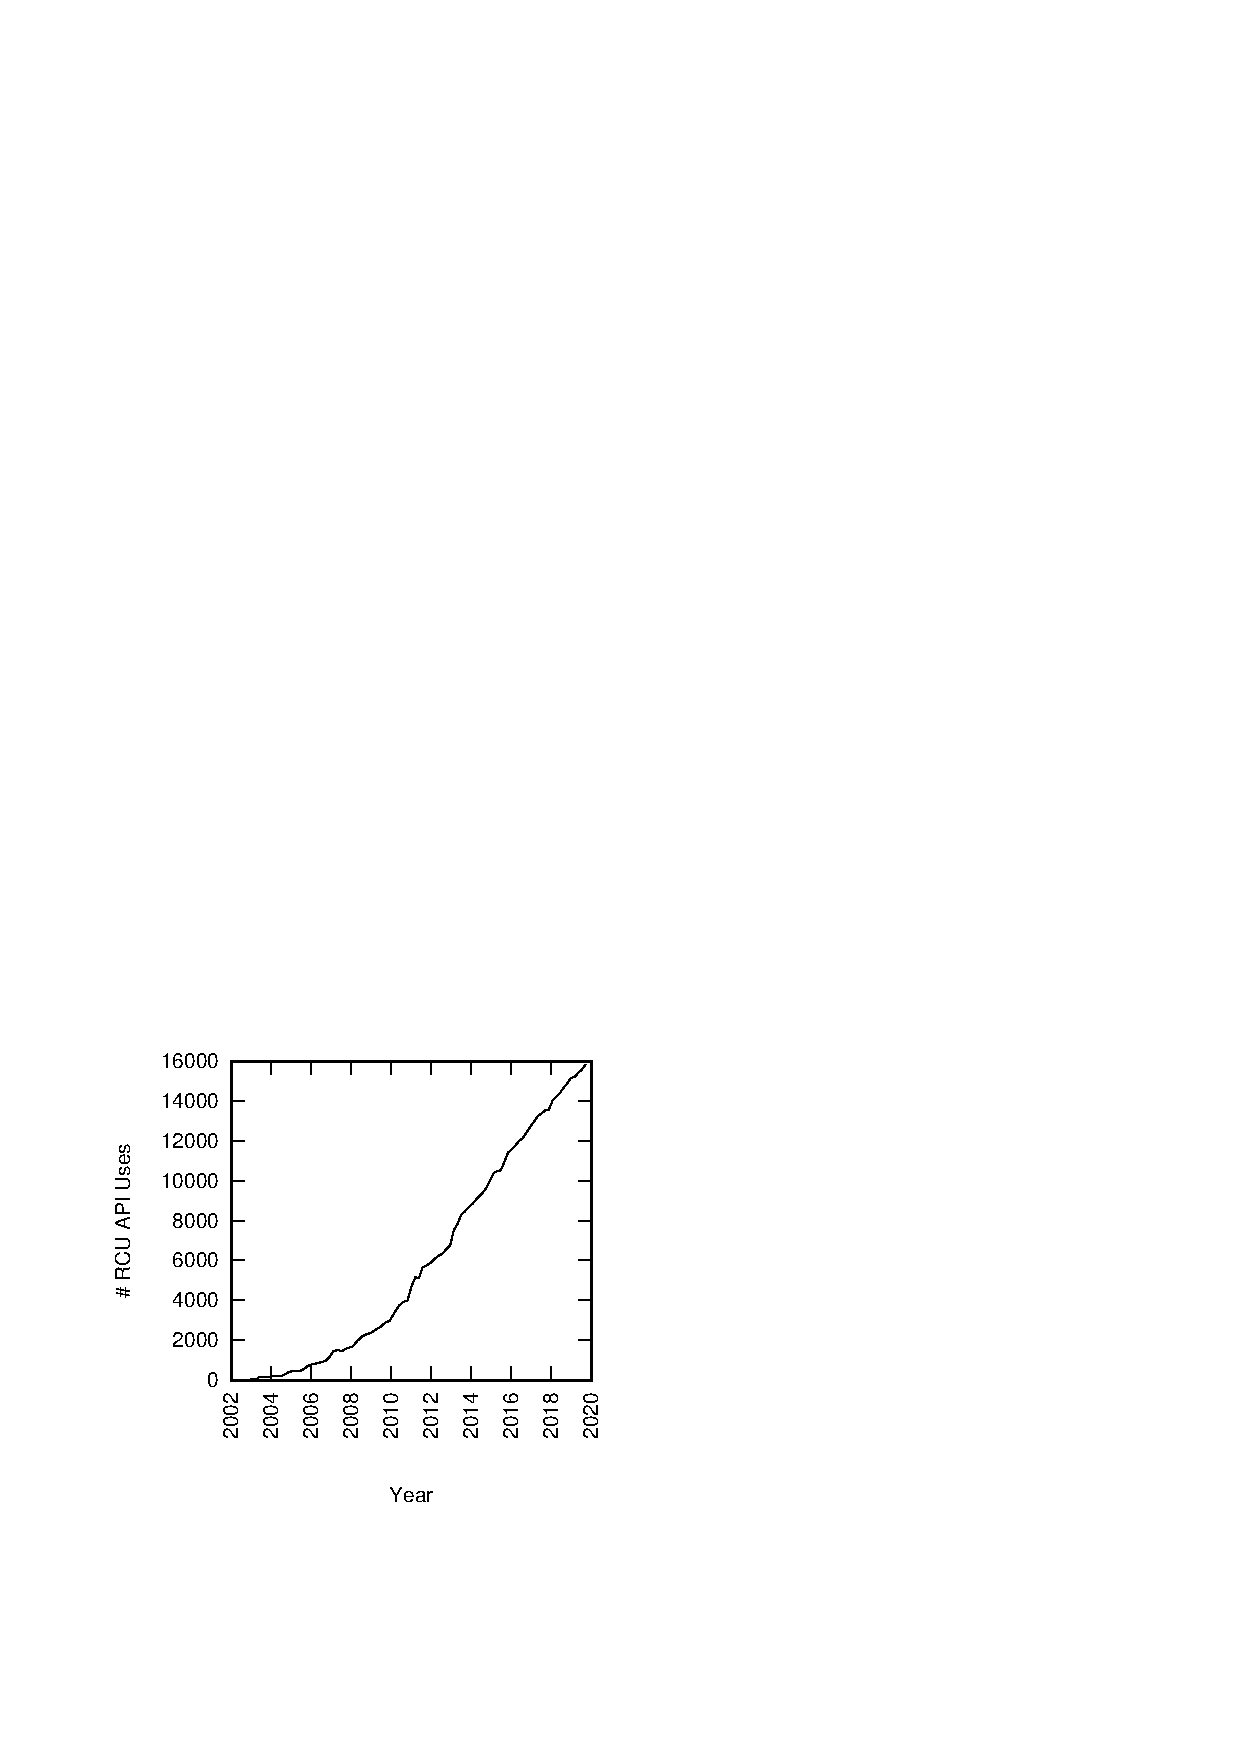
\includegraphics{defer/linux-RCU}}
\caption{RCU Usage in the Linux Kernel}
\label{fig:defer:RCU Usage in the Linux Kernel}
\end{figure}

RCU 는 2002년 10월 이래 리눅스 커널에서 사용되었습니다~\cite{Torvalds2.5.43}.
RCU API 의 사용은 그때 이후 상당히 늘어났는데,
Figure~\ref{fig:defer:RCU Usage in the Linux Kernel} 가 이를 잘 보이고
있습니다.
실제로,
Listing~\ref{lst:defer:Insertion and Deletion With Concurrent Readers}
의 것과 상당히 비슷한 코드가 리눅스 커널에 사용되었습니다.
\iffalse

It turns out that RCU has been used in the Linux kernel since
October 2002~\cite{Torvalds2.5.43}.
Use of the RCU API has increased substantially since that time,
as can be seen in
Figure~\ref{fig:defer:RCU Usage in the Linux Kernel}.
In fact, code very similar to that in
Listing~\ref{lst:defer:Insertion and Deletion With Concurrent Readers}
could be used in the Linux kernel.
\fi

그 전에는,  RCU 는 Sequent Computer System 의 DYNIX/ptx 운영체제에서 1990년대
초부터 사용되었습니다~\cite{McKenney98}, 그리고 그 전에는, 비슷한 메커니즘이
아마도 1980년대 중반부터 IBM 의 VM/XA 에서 사용되었습니다~\cite{Hennessy89}.
마지막으로,
Section~\ref{sec:defer:RCU Related Work} 에서 이야기 되었듯이, RCU 와 유사한
메커니즘들이 1980년대 초부터 학계와 산업계의 연구 분야 프로젝트들에서도
사용되었습니다~\cite{Kung80}, 그리고 보다 최근에는 다양한 유저스페이스
어플리케이션들에서도
사용되었습니다~\cite{MathieuDesnoyers2009URCU,MikeDay2013RCUqemu,GeoffRomer2018C++DeferredReclamationP0561R4}.
\iffalse

Prior to that, RCU was used in production in Sequent Computer Systems's
DYNIX/ptx operating system from the early 1990s~\cite{McKenney98},
and prior to that, a similar mechanism was used in IBM's
VM/XA, possibly as early as the mid-1980s~\cite{Hennessy89}.
Finally, as discussed in
Section~\ref{sec:defer:RCU Related Work},
mechanisms roughly similar to RCU have also been used
in academic and industrial-research projects as early as
1980~\cite{Kung80},
and more recently in production by a number of userspace
applications~\cite{MathieuDesnoyers2009URCU,MikeDay2013RCUqemu,GeoffRomer2018C++DeferredReclamationP0561R4}.
\fi

따라서 RCU 가 폭넓은 실용적 사용처를 가지고 있다고 말해도 됩니다.

이 섹션에서 다뤄진 최소한의 예제는 RCU 로의 좋은 소개가 됩니다.
하지만, RCU 의 효과적인 사용은 많은 경우 여러분이 여러분의 문제를 다르게 생각할
것을 필요로 합니다.
따라서 RCU 의 기본적인 사항들을 알아보는게 좋은데, 뒤따르는 섹션이 이를 도울
겁니다.
\iffalse

It is therefore safe to say that RCU enjoys wide practical applicability.

The minimal example discussed in this section is a good introduction to RCU.
However, effective use of RCU often requires that you think differently
about your problem.
It is therefore useful to examine RCU's fundamentals, a task taken up
by the following section.
\fi
